\documentclass[border=20pt]{standalone}
\newcounter{chapter} %dummy for import reasons
\usepackage{../../../mypackage}

\begin{document}
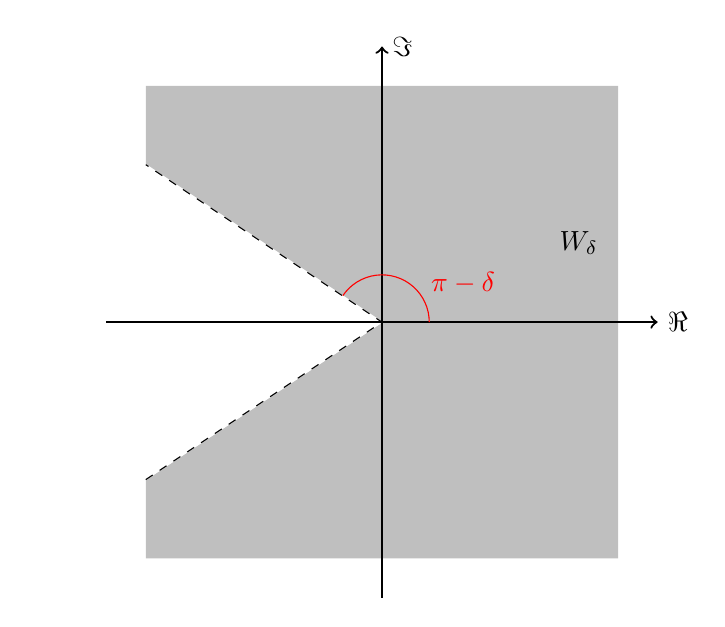
\begin{tikzpicture}
\fill [lightgray] (-3, -3) -- (-3, -2) -- (0, 0) -- (-3, 2) -- (-3, 3) -- (3,3) -- (3,-3) -- cycle;
%\path [inner color=gray, outer color=white] (0,0) circle (4);
%\fill [lightgray] (0,0) circle (3);
\fill [white] (-4.5, -3) -- (0, 0) -- (-4.5, 3) -- cycle;
\draw [white] (-3, -2) -- (0, 0) -- (-3,2);

% Achsen
\draw[thick, ->] (-3.5, 0) -- (3.5, 0) node[right] {$\Re$};
\draw[thick, ->] (0, -3.5) -- (0, 3.5) node[right] {$\Im$};

% 
\draw[dashed] (-3, -2) -- (0, 0) -- (-3, 2);
\draw [domain=0:146, red] plot ({0.6*cos(\x)}, {0.6*sin(\x)});
\draw (0.5,0.5) node [above, right, red] {$\pi - \delta$};
\node at (2.5,1) {$W_\delta$};
\end{tikzpicture}
\end{document}